\documentclass{standalone}

\usepackage{pgfplots}
\pgfplotsset{compat=1.16}

\begin{document}

% start
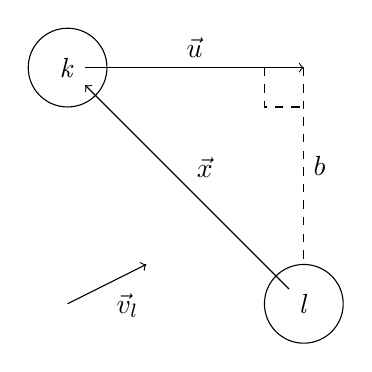
\begin{tikzpicture}
  \node(k) at (0,3) {\textit{k}};
  \node(l) at (3,0) {\textit{l}};
  \draw(k) circle [radius=0.5];
  \draw(l) circle [radius= 0.5];
  \draw[->](k) --(3,3) node
       [midway,above] {$\vec{u}$};
  \draw[->](l) -- (k) node
       [midway, above right]
       {$\vec{x}$};
  \draw[dashed] (3,3)--(3,0.5) node
       [midway, right] {$b$};
  \draw[dashed] (2.5,3)--(2.5,2.5)
       --(3,2.5);
  \draw[->] (0,0) -- (1,0.5) node
       [midway, below right]
       {$\vec{v}_l$};
\end{tikzpicture}
% end

\end{document}

